\documentclass[aspectratio=169]{beamer}

% ── Theme & Colors ──
\usetheme{Madrid}
\usecolortheme{whale}
\definecolor{darkblue}{RGB}{0,51,102}
\definecolor{accentblue}{RGB}{0,119,182}
\definecolor{lightgray}{RGB}{240,240,240}
\setbeamercolor{structure}{fg=darkblue}
\setbeamercolor{frametitle}{bg=darkblue,fg=white}
\setbeamercolor{title}{bg=darkblue,fg=white}
\setbeamercolor{block title}{bg=accentblue,fg=white}
\setbeamercolor{block body}{bg=lightgray,fg=black}
\setbeamercolor{item}{fg=accentblue}

\usepackage{graphicx}
\usepackage{amsmath,amssymb}
\usepackage{booktabs}
\usepackage{tikz}
\usetikzlibrary{shapes.geometric, arrows.meta, positioning, fit}

\setbeamerfont{title}{size=\large,series=\bfseries}
\setbeamerfont{frametitle}{size=\normalsize,series=\bfseries}

% ══════════════════════════════════════════════════════════
%                      TITLE PAGE
% ══════════════════════════════════════════════════════════
\title{AOC-IDS: Autonomous Online Framework with\\Contrastive Learning for Intrusion Detection}
\subtitle{IEEE INFOCOM 2024}
\author{\textbf{Pranav Inani}}
\institute{Paper by: X.\ Zhang, R.\ Zhao, Z.\ Jiang, Z.\ Sun, Y.\ Ding, E.C.H.\ Ngai, S.-H.\ Yang}
\date{\today}

\begin{document}

% ── Slide 1: Title ──
\begin{frame}[plain]
    \titlepage
\end{frame}

% ── Slide 2: Outline ──
\begin{frame}{Outline}
    \tableofcontents
\end{frame}

% ══════════════════════════════════════════════════════════
\section{Background \& Motivation}
% ══════════════════════════════════════════════════════════

\begin{frame}{The Problem with Traditional IDS}
    \begin{columns}[T]
        \begin{column}{0.55\textwidth}
            \textbf{Challenges in real-world intrusion detection:}
            \begin{itemize}
                \item Traditional IDS relies on \textbf{offline, static training}
                \item Attack strategies \textbf{evolve continuously}
                \item Manual labeling of network traffic is \textbf{expensive} and \textbf{slow}
                \item IoT environments generate \textbf{massive, dynamic} data streams
                \item Models degrade over time without retraining (\textbf{concept drift})
            \end{itemize}

            \vspace{0.4cm}
            \begin{block}{Key Question}
                How can an IDS \textit{autonomously} adapt to new traffic patterns \textit{without} human labeling?
            \end{block}
        \end{column}
        \begin{column}{0.42\textwidth}
            \centering
            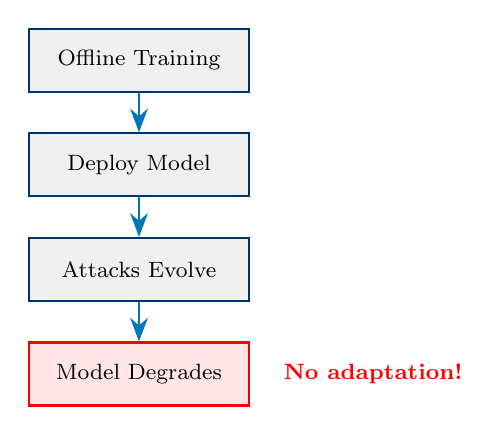
\begin{tikzpicture}[
                box/.style={rectangle, draw=darkblue, fill=lightgray, thick,
                            minimum width=2.8cm, minimum height=0.8cm, align=center,
                            font=\footnotesize},
                arr/.style={-{Stealth[length=3mm]}, thick, accentblue}
            ]
                \node[box] (train) {Offline Training};
                \node[box, below=0.5cm of train] (deploy) {Deploy Model};
                \node[box, below=0.5cm of deploy] (drift) {Attacks Evolve};
                \node[box, below=0.5cm of drift, draw=red, fill=red!10] (fail) {Model Degrades};

                \draw[arr] (train) -- (deploy);
                \draw[arr] (deploy) -- (drift);
                \draw[arr] (drift) -- (fail);

                \node[right=0.3cm of fail, font=\footnotesize\color{red}] {\textbf{No adaptation!}};
            \end{tikzpicture}
        \end{column}
    \end{columns}
\end{frame}

% ══════════════════════════════════════════════════════════
\section{AOC-IDS Framework}
% ══════════════════════════════════════════════════════════

\begin{frame}{AOC-IDS: System Overview}
    \centering
    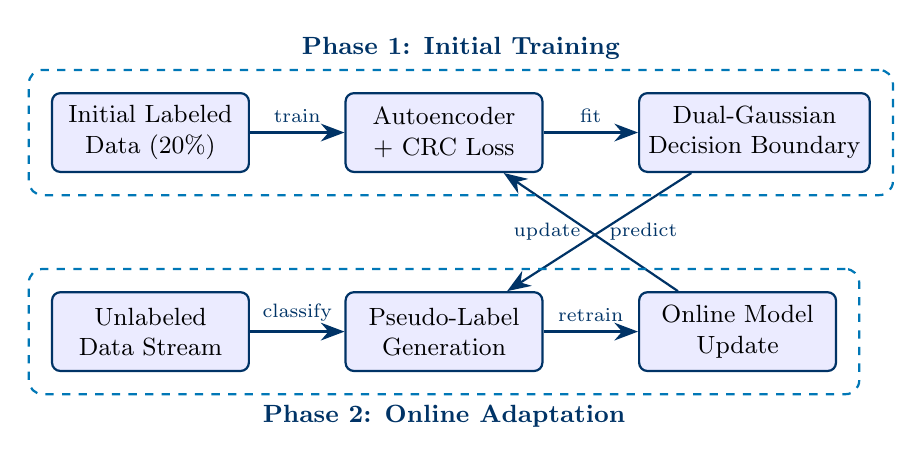
\begin{tikzpicture}[
        box/.style={rectangle, draw=darkblue, fill=blue!8, thick, rounded corners=3pt,
                    minimum width=2.5cm, minimum height=1cm, align=center,
                    font=\small},
        bigbox/.style={rectangle, draw=accentblue, thick, rounded corners=5pt,
                       inner sep=8pt, dashed},
        arr/.style={-{Stealth[length=3mm]}, thick, darkblue},
        lbl/.style={font=\scriptsize\color{accentblue}, midway}
    ]
        % Phase 1
        \node[box] (data) {Initial Labeled\\Data (20\%)};
        \node[box, right=1.2cm of data] (ae) {Autoencoder\\+ CRC Loss};
        \node[box, right=1.2cm of ae] (gmm) {Dual-Gaussian\\Decision Boundary};

        % Phase 2
        \node[box, below=1.5cm of data] (stream) {Unlabeled\\Data Stream};
        \node[box, right=1.2cm of stream] (pseudo) {Pseudo-Label\\Generation};
        \node[box, right=1.2cm of pseudo] (update) {Online Model\\Update};

        \draw[arr] (data) -- (ae) node[lbl, above] {train};
        \draw[arr] (ae) -- (gmm) node[lbl, above] {fit};
        \draw[arr] (stream) -- (pseudo) node[lbl, above] {classify};
        \draw[arr] (pseudo) -- (update) node[lbl, above] {retrain};
        \draw[arr] (gmm) -- (pseudo) node[lbl, right] {predict};
        \draw[arr] (update) -- (ae) node[lbl, left] {update};

        % Phase labels
        \node[bigbox, fit=(data)(ae)(gmm), label={[font=\small\bfseries\color{darkblue}]above:Phase 1: Initial Training}] {};
        \node[bigbox, fit=(stream)(pseudo)(update), label={[font=\small\bfseries\color{darkblue}]below:Phase 2: Online Adaptation}] {};
    \end{tikzpicture}
\end{frame}

\begin{frame}{Core Component: Autoencoder + CRC Loss}
    \begin{columns}[T]
        \begin{column}{0.48\textwidth}
            \textbf{Autoencoder Architecture}
            \begin{itemize}
                \item Encoder: $d \to d/2 \to d/4$ (bottleneck)
                \item Decoder: $d/4 \to d/2 \to d$ (reconstruction)
                \item Outputs \textbf{two} representation spaces:
                \begin{itemize}
                    \item Encoder embeddings (compressed features)
                    \item Decoder reconstructions
                \end{itemize}
            \end{itemize}

            \vspace{0.3cm}
            \textbf{Total Loss:}
            \[
                \mathcal{L} = \mathcal{L}_{\text{CRC}}^{\text{encoder}} + \mathcal{L}_{\text{CRC}}^{\text{decoder}}
            \]
        \end{column}
        \begin{column}{0.48\textwidth}
            \textbf{Cluster Repelling Contrastive (CRC) Loss}
            \begin{itemize}
                \item Based on InfoNCE, but with \textbf{two traversals} of the abnormal set
                \item Pulls normal samples \textbf{together}
                \item Pushes normal and abnormal samples \textbf{apart}
            \end{itemize}

            \vspace{0.2cm}
            \[
                \mathcal{L}_{\text{CRC}} = -\frac{1}{N_n}\sum_{i \in \mathcal{N}} \log \frac{e^{s_{ij}/\tau}}{e^{s_{ij}/\tau} + \sum_{k \in \mathcal{A}} e^{s_{ik}/\tau}}
            \]

            \vspace{0.1cm}
            {\scriptsize where $s_{ij}$ = cosine similarity, $\tau$ = temperature, $\mathcal{N}$ = normal, $\mathcal{A}$ = abnormal}
        \end{column}
    \end{columns}
\end{frame}

\begin{frame}{Detection: Dual-Gaussian Decision Boundary}
    \begin{columns}[T]
        \begin{column}{0.52\textwidth}
            \textbf{How detection works:}
            \begin{enumerate}
                \item Compute \textbf{normal template} = mean embedding of all normal training samples
                \item For each sample, compute \textbf{cosine similarity} to normal template
                \item Fit \textbf{two Gaussians} (via MLE) to the similarity distribution:
                \begin{itemize}
                    \item $\mathcal{N}(\mu_1, \sigma_1)$ — normal cluster (high similarity)
                    \item $\mathcal{N}(\mu_2, \sigma_2)$ — abnormal cluster (low similarity)
                \end{itemize}
                \item Classify: if $p(\text{abnormal} \mid x) > p(\text{normal} \mid x)$ $\Rightarrow$ \textbf{attack}
            \end{enumerate}

            \vspace{0.2cm}
            \textbf{Final vote:} encoder and decoder predictions combined by confidence ($|p_1 - p_2|$).
        \end{column}
        \begin{column}{0.44\textwidth}
            \centering
            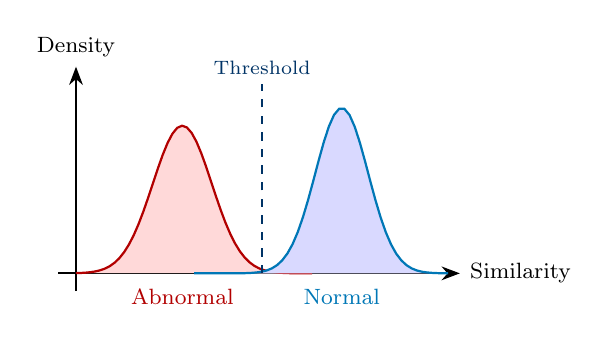
\begin{tikzpicture}[scale=0.75]
                % Axes
                \draw[-{Stealth}, thick] (-0.3,0) -- (6.5,0) node[right, font=\footnotesize] {Similarity};
                \draw[-{Stealth}, thick] (0,-0.3) -- (0,3.5) node[above, font=\footnotesize] {Density};

                % Gaussian 1 (abnormal, left)
                \draw[thick, red!70!black, fill=red!15]
                    plot[domain=0:4, samples=50] (\x, {2.5*exp(-(\x-1.8)^2/0.5)});
                \node[font=\footnotesize, red!70!black] at (1.8, -0.4) {Abnormal};

                % Gaussian 2 (normal, right)
                \draw[thick, accentblue, fill=blue!15]
                    plot[domain=2:6.3, samples=50] (\x, {2.8*exp(-(\x-4.5)^2/0.4)});
                \node[font=\footnotesize, accentblue] at (4.5, -0.4) {Normal};

                % Decision boundary
                \draw[thick, dashed, darkblue] (3.15, 0) -- (3.15, 3.2)
                    node[above, font=\scriptsize] {Threshold};
            \end{tikzpicture}
        \end{column}
    \end{columns}
\end{frame}

\begin{frame}{Online Pseudo-Labeling Loop}
    \begin{columns}[T]
        \begin{column}{0.55\textwidth}
            \textbf{How online adaptation works:}
            \begin{enumerate}
                \item Start with a small labeled set (20\% of training data)
                \item Train the AE + CRC model on this initial set
                \item Receive a \textbf{chunk} of unlabeled data (size = \texttt{sample\_interval})
                \item Use Gaussian decision boundary to \textbf{predict pseudo-labels}
                \item \textbf{Flip} a small fraction of labels (5\%) for robustness
                \item Add pseudo-labeled data to training set
                \item \textbf{Retrain} model for \texttt{epoch\_1} epochs
                \item Repeat until all data is consumed
            \end{enumerate}
        \end{column}
        \begin{column}{0.42\textwidth}
            \centering
            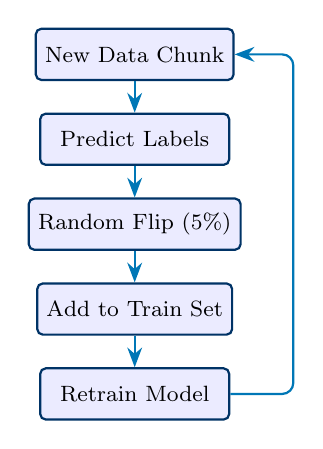
\begin{tikzpicture}[
                box/.style={rectangle, draw=darkblue, fill=blue!8, thick,
                            rounded corners=2pt, minimum width=2.4cm,
                            minimum height=0.65cm, align=center, font=\footnotesize},
                arr/.style={-{Stealth[length=2.5mm]}, thick, accentblue}
            ]
                \node[box] (chunk) {New Data Chunk};
                \node[box, below=0.4cm of chunk] (pred) {Predict Labels};
                \node[box, below=0.4cm of pred] (flip) {Random Flip (5\%)};
                \node[box, below=0.4cm of flip] (add) {Add to Train Set};
                \node[box, below=0.4cm of add] (train) {Retrain Model};

                \draw[arr] (chunk) -- (pred);
                \draw[arr] (pred) -- (flip);
                \draw[arr] (flip) -- (add);
                \draw[arr] (add) -- (train);
                \draw[arr, rounded corners] (train.east) -- ++(0.8,0) |- (chunk.east);
            \end{tikzpicture}
        \end{column}
    \end{columns}
\end{frame}

\begin{frame}{Experimental Results}
    \begin{columns}[T]
        \begin{column}{0.48\textwidth}
            \textbf{Datasets:}
            \begin{itemize}
                \item \textbf{NSL-KDD} — 121 features, binary labels
                \item \textbf{UNSW-NB15} — 196 features, binary labels
                \item Preprocessed: normalized continuous, one-hot categorical
            \end{itemize}

            \vspace{0.3cm}
            \textbf{Setup:}
            \begin{itemize}
                \item 20\% initial labeled data
                \item 80\% arrives as unlabeled stream
                \item 5 random seeds, averaged results
                \item Evaluated: Accuracy, Precision, Recall, F1
            \end{itemize}
        \end{column}
        \begin{column}{0.48\textwidth}
            \textbf{Key findings from the paper:}
            \begin{itemize}
                \item AOC-IDS \textbf{outperforms} state-of-the-art on both datasets
                \item Achieves strong results with \textbf{only 20\%} labeled data
                \item Online adaptation \textbf{improves} performance over the static baseline
                \item CRC loss is \textbf{more effective} than standard contrastive losses (InfoNCE)
            \end{itemize}

            \vspace{0.2cm}
            \begin{block}{Significance}
                First framework combining contrastive learning with autonomous online adaptation for IDS.
            \end{block}
        \end{column}
    \end{columns}
\end{frame}

% ══════════════════════════════════════════════════════════
\section{Our Novel Contributions}
% ══════════════════════════════════════════════════════════

\begin{frame}{Novelty 1: GMM-Based Adaptive Decision Boundary}
    \begin{columns}[T]
        \begin{column}{0.48\textwidth}
            \textbf{Problem with original approach:}
            \begin{itemize}
                \item Fixed \textbf{2-Gaussian} assumption
                \item Multiple attack types (DDoS, Probe, R2L\ldots) form \textbf{different clusters}
                \item Nelder-Mead optimizer is \textbf{unconstrained} — can produce negative $\sigma$
            \end{itemize}

            \vspace{0.3cm}
            \textbf{Our improvement:}
            \begin{itemize}
                \item Replace with \textbf{Gaussian Mixture Model (GMM)}
                \item Auto-select components ($k=2{\text{-}}5$) via \textbf{BIC}
                \item Label components as normal/abnormal using \textbf{training label majority}
                \item Posterior probabilities give natural \textbf{confidence scores}
            \end{itemize}
        \end{column}
        \begin{column}{0.48\textwidth}
            \centering
            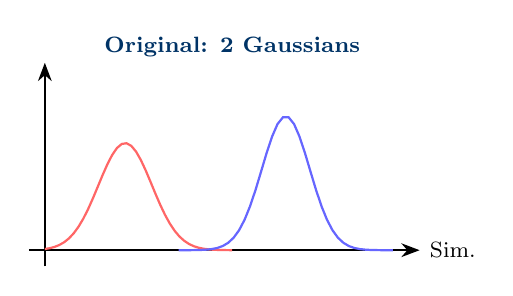
\begin{tikzpicture}[scale=0.68]
                \draw[-{Stealth}, thick] (-0.3,0) -- (7,0) node[right, font=\footnotesize] {Sim.};
                \draw[-{Stealth}, thick] (0,-0.3) -- (0,3.5);

                % Original: 2 Gaussians
                \node[font=\footnotesize\bfseries, darkblue] at (3.5, 3.8) {Original: 2 Gaussians};
                \draw[thick, red!60] plot[domain=0:3.5, samples=40]
                    (\x, {2*exp(-(\x-1.5)^2/0.5)});
                \draw[thick, blue!60] plot[domain=2.5:6.5, samples=40]
                    (\x, {2.5*exp(-(\x-4.5)^2/0.4)});
            \end{tikzpicture}

            \vspace{0.2cm}

            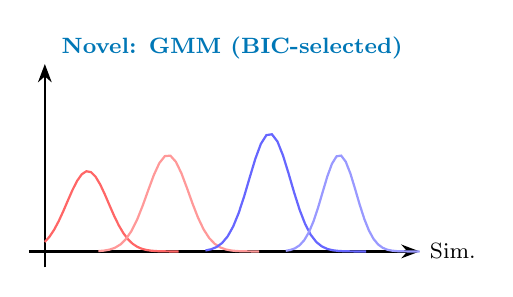
\begin{tikzpicture}[scale=0.68]
                \draw[-{Stealth}, thick] (-0.3,0) -- (7,0) node[right, font=\footnotesize] {Sim.};
                \draw[-{Stealth}, thick] (0,-0.3) -- (0,3.5);

                % Novel: GMM with 4 components
                \node[font=\footnotesize\bfseries, accentblue] at (3.5, 3.8) {Novel: GMM (BIC-selected)};
                \draw[thick, red!60] plot[domain=0:2.5, samples=30]
                    (\x, {1.5*exp(-(\x-0.8)^2/0.3)});
                \draw[thick, red!40] plot[domain=1:4, samples=30]
                    (\x, {1.8*exp(-(\x-2.3)^2/0.3)});
                \draw[thick, blue!60] plot[domain=3:6, samples=30]
                    (\x, {2.2*exp(-(\x-4.2)^2/0.3)});
                \draw[thick, blue!40] plot[domain=4.5:7, samples=30]
                    (\x, {1.8*exp(-(\x-5.5)^2/0.2)});
            \end{tikzpicture}
        \end{column}
    \end{columns}
\end{frame}

\begin{frame}{Novelty 2: Confidence-Aware Pseudo-Label Filtering}
    \begin{columns}[T]
        \begin{column}{0.48\textwidth}
            \textbf{Problem with original approach:}
            \begin{itemize}
                \item \textbf{All} pseudo-labels added to training — including wrong ones
                \item Random flipping (5\%) is \textbf{blind}: flips correct labels too
                \item Noisy labels \textbf{accumulate} over online rounds
                \item Model performance degrades with error propagation
            \end{itemize}

            \vspace{0.3cm}
            \textbf{Our improvement:}
            \begin{itemize}
                \item Compute \textbf{confidence} = $|P(\text{normal}) - P(\text{abnormal})|$ from GMM posteriors
                \item Only add samples with confidence $\geq \theta$ to training
                \item \textbf{Eliminate} random flipping entirely
                \item Separate \textbf{evaluation pool} (all data) from \textbf{training pool} (confident only)
            \end{itemize}
        \end{column}
        \begin{column}{0.48\textwidth}
            \centering
            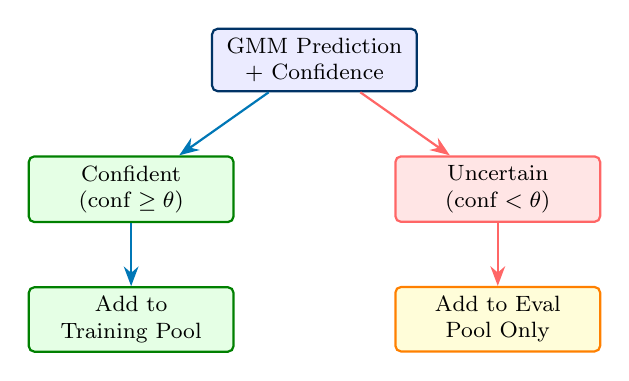
\begin{tikzpicture}[
                box/.style={rectangle, draw=darkblue, fill=blue!8, thick,
                            rounded corners=2pt, minimum width=2.6cm,
                            minimum height=0.6cm, align=center, font=\footnotesize},
                arr/.style={-{Stealth[length=2.5mm]}, thick, accentblue},
                redarr/.style={-{Stealth[length=2.5mm]}, thick, red!60}
            ]
                \node[box] (pred) {GMM Prediction\\+ Confidence};
                \node[box, below left=0.8cm and -0.3cm of pred, fill=green!10, draw=green!50!black]
                    (conf) {Confident\\(conf $\geq \theta$)};
                \node[box, below right=0.8cm and -0.3cm of pred, fill=red!10, draw=red!60]
                    (unconf) {Uncertain\\(conf $< \theta$)};
                \node[box, below=0.8cm of conf, fill=green!10, draw=green!50!black]
                    (train) {Add to\\Training Pool};
                \node[box, below=0.8cm of unconf, fill=yellow!15, draw=orange]
                    (eval) {Add to Eval\\Pool Only};

                \draw[arr] (pred) -- (conf);
                \draw[redarr] (pred) -- (unconf);
                \draw[arr] (conf) -- (train);
                \draw[redarr] (unconf) -- (eval);
            \end{tikzpicture}

            \vspace{0.3cm}
            {\footnotesize \textbf{Result:} Cleaner training data $\Rightarrow$ better model $\Rightarrow$ better future predictions (virtuous cycle)}
        \end{column}
    \end{columns}
\end{frame}

\begin{frame}{Novelty 3: Dynamic Temperature Scheduling}
    \begin{columns}[T]
        \begin{column}{0.48\textwidth}
            \textbf{Problem with original approach:}
            \begin{itemize}
                \item Fixed temperature $\tau = 0.02$ throughout training
                \item Too aggressive early on (embeddings still forming)
                \item Same $\tau$ for initial and online phases, but they have \textbf{different needs}
            \end{itemize}

            \vspace{0.3cm}
            \textbf{Our improvement — Cosine Annealing:}
            \[
                \tau(t) = \tau_{\min} + \frac{\tau_{\max} - \tau_{\min}}{2}\left(1 + \cos\frac{\pi\, t}{T}\right)
            \]
            \begin{itemize}
                \item \textbf{Phase 1} (initial): $\tau$ anneals from 0.1 $\to$ 0.02
                    \begin{itemize}
                        \item[\footnotesize$\triangleright$] Soft contrasts early, sharp contrasts later
                    \end{itemize}
                \item \textbf{Phase 2} (online): fixed $\tau = 0.05$ (warmer)
                    \begin{itemize}
                        \item[\footnotesize$\triangleright$] Prevents overfitting to noisy pseudo-labels
                    \end{itemize}
            \end{itemize}
        \end{column}
        \begin{column}{0.48\textwidth}
            \centering
            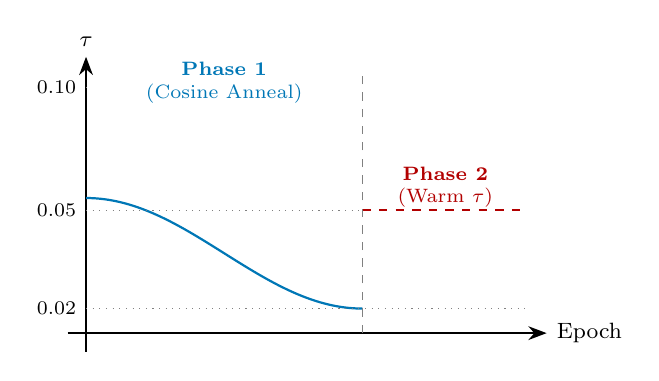
\begin{tikzpicture}[scale=0.78]
                % Axes
                \draw[-{Stealth}, thick] (-0.3,0) -- (7.5,0) node[right, font=\footnotesize] {Epoch};
                \draw[-{Stealth}, thick] (0,-0.3) -- (0,4.5) node[above, font=\footnotesize] {$\tau$};

                % Y-axis labels
                \node[left, font=\scriptsize] at (0, 0.4) {0.02};
                \node[left, font=\scriptsize] at (0, 2.0) {0.05};
                \node[left, font=\scriptsize] at (0, 4.0) {0.10};

                % Phase 1: cosine annealing
                \draw[thick, accentblue]
                    plot[domain=0:4.5, samples=60]
                    (\x, {0.4 + 1.8*(1 + cos(deg(\x*3.14159/4.5)))/2});

                % Phase 2: flat warm temp
                \draw[thick, red!70!black, dashed] (4.5, 2.0) -- (7.2, 2.0);

                % Phase separator
                \draw[thin, gray, dashed] (4.5, 0) -- (4.5, 4.3);

                % Labels
                \node[font=\scriptsize, accentblue] at (2.25, 4.3) {\textbf{Phase 1}};
                \node[font=\scriptsize, accentblue] at (2.25, 3.9) {(Cosine Anneal)};
                \node[font=\scriptsize, red!70!black] at (5.85, 2.6) {\textbf{Phase 2}};
                \node[font=\scriptsize, red!70!black] at (5.85, 2.2) {(Warm $\tau$)};

                % Dotted guide lines
                \draw[dotted, gray] (0, 0.4) -- (7.2, 0.4);
                \draw[dotted, gray] (0, 2.0) -- (4.5, 2.0);
                \draw[dotted, gray] (0, 4.0) -- (0.1, 4.0);
            \end{tikzpicture}

            \vspace{0.3cm}
            {\footnotesize High $\tau$ = soft separation (exploration)\\
            Low $\tau$ = hard separation (exploitation)}
        \end{column}
    \end{columns}
\end{frame}

% ══════════════════════════════════════════════════════════
\section{Summary}
% ══════════════════════════════════════════════════════════

\begin{frame}{Summary of Contributions}
    \begin{table}[h]
        \centering
        \renewcommand{\arraystretch}{1.3}
        \begin{tabular}{@{}lll@{}}
            \toprule
            \textbf{Aspect} & \textbf{Original AOC-IDS} & \textbf{Our Improvement} \\
            \midrule
            Decision Boundary & Fixed 2-Gaussian MLE & GMM with BIC selection \\
            Pseudo-Label Quality & Random flip (5\%) & Confidence-based filtering \\
            CRC Temperature & Fixed $\tau = 0.02$ & Cosine annealing + warm online $\tau$ \\
            \bottomrule
        \end{tabular}
    \end{table}

    \vspace{0.4cm}

    \begin{block}{Why These Improvements Matter}
        \begin{itemize}
            \item \textbf{GMM}: Captures multi-modal attack distributions $\Rightarrow$ better boundaries
            \item \textbf{Confidence filtering}: Breaks error propagation cycle $\Rightarrow$ cleaner online learning
            \item \textbf{Temperature scheduling}: Matches training dynamics $\Rightarrow$ stable convergence
        \end{itemize}
    \end{block}

    \vspace{0.3cm}
    \centering
    {\large\textbf{Thank You!}}\\[0.2cm]
    {\footnotesize Code: \texttt{novel\_online\_training.py} \quad|\quad \texttt{novel\_utils.py}}
\end{frame}

\end{document}
